\documentclass[conference]{IEEEtran}
\IEEEoverridecommandlockouts

\usepackage{cite}
\usepackage{amsmath,amssymb,amsfonts}
\usepackage{graphicx}
\usepackage{textcomp}
\usepackage{xcolor}
\usepackage{booktabs}
\usepackage{array}
\usepackage{url}
\usepackage{tabularx}
\usepackage{multirow}
\usepackage{makecell}

\graphicspath{{../../clean-pipeline-56-32/outputs/figures/}{../../notebooks/kaggle_outputs_proof05/}{../../notebooks/final_clustering_outputs06/}{../../figures/}{./}}

% --- Mengurangi warning underfull/overfull hbox ---
\tolerance=1000
\emergencystretch=1em
\hbadness=10000
\vbadness=10000

\def\BibTeX{{\rm B\kern-.05em{\sc i\kern-.025em b}\kern-.08em
    T\kern-.1667em\lower.7ex\hbox{E}\kern-.125emX}}

\newcolumntype{Y}{>{\raggedright\arraybackslash}X}
\newcolumntype{P}[1]{>{\centering\arraybackslash}p{#1}}
\newcolumntype{R}{>{\raggedleft\arraybackslash}p{1.0cm}}

\begin{document}

% ============================================================
% JUDUL & AUTHOR
% ============================================================
\title{Impact of Feature Scaling and Temporal Window Aggregation on Multivariate Geothermal Drilling Sensor Clustering Using K-Means}

\author{
\begin{tabular}{ccc}
    \textbf{Aulia Fadhila Mumtaza} & \textbf{Fathan Ariiq Rasbi Yalsi} & \textbf{Achmad Faruq Mahdison} \\
    \textit{Teknik Informatika} & \textit{Teknik Informatika} & \textit{Teknik Informatika} \\
    \textit{Universitas Padjadjaran} & \textit{Universitas Padjadjaran} & \textit{Universitas Padjadjaran} \\
    Sumedang, Indonesia & Sumedang, Indonesia & Sumedang, Indonesia \\
    aulia24014@mail.unpad.ac.id & fathan24002@mail.unpad.ac.id & achmad24007@mail.unpad.ac.id \\[1.5em]
    \multicolumn{3}{c}{%
        \begin{tabular}{cc}
            \textbf{Aliya Zahra Nurazizah} & \textbf{M Rafif Widyadhana} \\
            \textit{Teknik Informatika} & \textit{Teknik Informatika} \\
            \textit{Universitas Padjadjaran} & \textit{Universitas Padjadjaran} \\
            Sumedang, Indonesia & Sumedang, Indonesia \\
            aliya24007@mail.unpad.ac.id & mrafif24001@mail.unpad.ac.id \\
        \end{tabular}%
    } \\
\end{tabular}
}

\maketitle

% ============================================================
% ABSTRAK
% ============================================================
\begin{abstract}
Data sensor rig pengeboran geotermal berfrekuensi 1 Hz bersifat multivariat, tidak berlabel, berskala timpang, dan memiliki autokorelasi serial yang kuat ($r \approx 1{,}0$). Makalah ini menyajikan kerangka kerja klasterisasi deret waktu tanpa kebocoran informasi (\textit{leakage-free}) pada 2.506.359 rekaman sensor sumur Utah FORGE 56-32 menggunakan K-Means dan Gaussian Mixture Models (GMM) pada 13 kanal sensor (11 sensor mentah dan 2 proksi daya fisik) yang diringkas ke dalam 39 fitur statistik jendela geser. Protokol pra-pemrosesan mencakup eliminasi anomali SPP ($\le -900$ psi; 29.503 baris), \textit{masking} kode sentinel $-999{,}25$ menjadi NaN, segmentasi adaptif berbasis celah waktu, serta jendela \textit{tumbling} 60 detik (stride 60 s, 0\% tumpang-tindih) dengan ambang kelengkapan data $\ge 90\%$. Evaluasi eksperimental berbasis partisi kronologis (Train 70\% / Test 30\%) dengan embargo 1 jam serta \textit{guardrail} ketat menghasilkan empat temuan fundamental. Pertama, pengujian membongkar ilusi metrik internal konvensional: \textit{RobustScaler} menghasilkan skor \textit{Silhouette} semu yang tinggi ($0{,}8822$ Train / $0{,}8557$ Test) namun mengalami keruntuhan klaster katastropik (\textit{cluster collapse}) di mana 99{,}25\% data menumpuk pada satu klaster (\textit{NO-WINNER}). Kedua, \textit{MinMaxScaler} terbukti sebagai satu-satunya skenario yang stabil dan lolos seluruh aturan baku (\textit{ELIGIBLE}) dengan \textit{Silhouette} $0{,}3104$ (Train) dan $0{,}2677$ (Test), DBI $1{,}5715$ (Train) dan $2{,}0611$ (Test), serta kestabilan stokastik ARI $0{,}9997$. Ketiga, representasi jendela 60 detik mereduksi osilasi peralihan label (\textit{label chattering}) sebesar delapan kali lipat dari $0{,}0102$ menjadi $0{,}0013$ kedipan/detik, selaras dengan konstanta respons hidraulik formasi granit. Keempat, penelusuran $k=2..8$ menetapkan $k=4$ sebagai konfigurasi optimal K-Means yang membagi data secara berimbang ke dalam empat klaster operasional rig: \textit{active drilling} (34{,}63\%), \textit{high-pressure resistant drilling} (39{,}94\%), \textit{circulation \& hole cleaning} (13{,}07\%), dan \textit{pipe connection/slips standby} (12{,}36\%).
\end{abstract}

\begin{IEEEkeywords}
klasterisasi deret waktu, K-Means, sensor pengeboran geotermal, MinMaxScaler, jendela geser, anti-kebocoran data, Utah FORGE
\end{IEEEkeywords}

% ============================================================
% I. PENDAHULUAN
% ============================================================
\section{Pendahuluan}

\subsection{Permasalahan Data Sensor Multivariat}
Pemantauan operasional rig pengeboran panas bumi skala besar, seperti pada sumur Utah FORGE 56-32, menghasilkan rekaman data sensor deret waktu berdimensi tinggi (\textit{multivariate time-series}) dengan frekuensi pencatatan 1 Hz (satu observasi per detik). Dataset historis yang berukuran sangat masif ini merekam dinamika parameter mekanika dan hidraulika pengeboran tanpa disertai anotasi kejadian operasional (\textit{unlabeled data}). Oleh karena itu, pengenalan rezim operasi rig (seperti \textit{active drilling}, \textit{circulation}, \textit{tripping}, dan \textit{idle}) membutuhkan pendekatan pembelajaran mesin tak terawasi (\textit{unsupervised learning}) seperti klasterisasi K-Means.

Namun, pemrosesan aliran data sensor industri mentah menghadirkan tiga tantangan teknis fundamental yang berpotensi membiaskan pemodelan klasterisasi jika tidak ditangani secara analitis:

\begin{enumerate}
\item \textbf{Ketimpangan Skala Lintas Orde Besaran (\textit{Scale Disparity}):} Terdapat perbedaan rentang nilai numerik yang sangat ekstrem antar-sensor. Sensor hidraulik seperti \textit{Standpipe Pressure} (SPP) beroperasi pada orde ribuan (0--3.500 psi), sedangkan sensor kinetik seperti \textit{Rotary Torque} hanya bernilai puluhan (0--15 kft$\cdot$lb). Analisis variansi menunjukkan bahwa SPP dan \textit{Total Pump Output} mendominasi hingga 99{,}36\% dari total variansi sistem. Jika tidak dikalibrasi, metrik jarak \textit{Euclidean} akan secara absolut menenggelamkan sensor mekanik, sehingga algoritma praktis hanya mengklasifikasikan tekanan pompa.

\item \textbf{Ketergantungan Waktu (\textit{Temporal Dependency}):} Fluktuasi nilai sensor industri tidak bersifat saling lepas (\textit{independent}). Pencatatan berfrekuensi 1 Hz memiliki tingkat keterikatan urutan waktu yang sangat kuat, dibuktikan dengan nilai autokorelasi lag-1 yang bertengger di atas koefisien 0{,}95. Pemrosesan data secara titik tunggal (\textit{point-based clustering}) terbukti akan memicu pergantian transisi label klaster yang tidak rasional (\textit{chattering} atau \textit{flickering}) tiap detiknya, serta menghilangkan konteks tren dinamika gerak mesin.

\item \textbf{Derau Sistemik dan Pencilan Ekstrem (\textit{Systemic Noise and Outliers}):} Anomali instrumen terekam dalam dua bentuk. Pertama, ketiadaan data sistemik (seperti pada sensor Gas dan \textit{Gamma Ray}) yang memunculkan nilai sentinel statis $-999{,}25$. Kedua, pencilan transien fisik (artefak), di mana variabel laju penembusan (\textit{Rate of Penetration} / ROP) mencatatkan lonjakan palsu hingga 11.145 ft/jam saat rangkaian mata bor sedang melayang di udara (\textit{off-bottom}). Selain itu, variabel \textit{Differential Pressure} memunculkan kecacatan kalkulasi bernilai negatif ($\le -900$ psi) saat pompa dimatikan.
\end{enumerate}

\subsection{Validasi Kuantitatif Ketiga Tantangan}
Ketiga tantangan teoretis tersebut terbukti secara kuantitatif hadir di dalam dataset Utah FORGE 56-32. Eksplorasi statistik awal yang telah dilakukan menunjukkan bahwa ketimpangan skala benar-benar terjadi, di mana satu sensor mendominasi 52{,}68\% total variansi dengan rasio rentang antar-sensor mencapai 348{,}9 kali lipat (ROP terhadap Torque). Ketergantungan waktu tervalidasi melalui uji autokorelasi lag-1, di mana sensor utama seperti tekanan hidraulik, putaran, dan laju penetrasi mencatatkan skor keterikatan waktu yang nyaris sempurna, masing-masing 0{,}9998; 0{,}9990; dan 0{,}9884. Terakhir, masalah derau dan pencilan terekam nyata dengan adanya persentase data mati (kode sentinel $-999{,}25$) sebesar $\sim 1{,}17\%$, serta kerusakan sebaran data akibat lonjakan kecepatan pengeboran palsu dengan nilai kemiringan (\textit{skewness}) yang sangat ekstrem hingga mencapai angka 23{,}54. Bukti-bukti matematis inilah yang mendasari diperlukannya tahap pra-pemrosesan data secara komprehensif sebelum pemodelan dilakukan.

\subsection{Tinjauan Pustaka Sistematis (PRISMA)}
Untuk merumuskan strategi penanganan data (\textit{data preprocessing}) yang optimal dan divalidasi secara saintifik, penelitian ini merujuk pada pedoman tinjauan literatur sistematis PRISMA 2020 (\textit{Preferred Reporting Items for Systematic Reviews and Meta-Analyses}). Tahapan seleksi dilakukan dalam empat fase utama:

\begin{enumerate}
\item \textbf{Identifikasi:} Pencarian awal pada basis data akademik utama (Scopus dan IEEE Xplore) dalam rentang publikasi 2016 hingga 2026. Kata kunci yang digunakan mengiriskan domain \textit{``multivariate time-series''}, \textit{``K-Means clustering''}, \textit{``data preprocessing''}, dan \textit{``industrial sensor data''}.
\item \textbf{Penyaringan:} Menyaring duplikasi dari ratusan hasil pencarian awal, dilanjutkan dengan pemindaian judul dan abstrak untuk mengeliminasi studi yang tidak berfokus pada data tak berlabel (\textit{unsupervised}).
\item \textbf{Uji Kelayakan:} Enam belas artikel teks penuh (\textit{full-text}) dievaluasi secara mendalam. Delapan dokumen dieksklusi karena ketidaksesuaian domain fisik operasional (seperti analisis regangan tektonik gempa bumi, sinyal emisi akustik frekuensi tinggi, atau EOR kimiawi tanpa klasterisasi deret waktu).
\item \textbf{Inklusi:} Menetapkan delapan literatur acuan utama yang paling selaras secara metodologis menjadi landasan.
\end{enumerate}

\begin{figure}[!t]
\centering
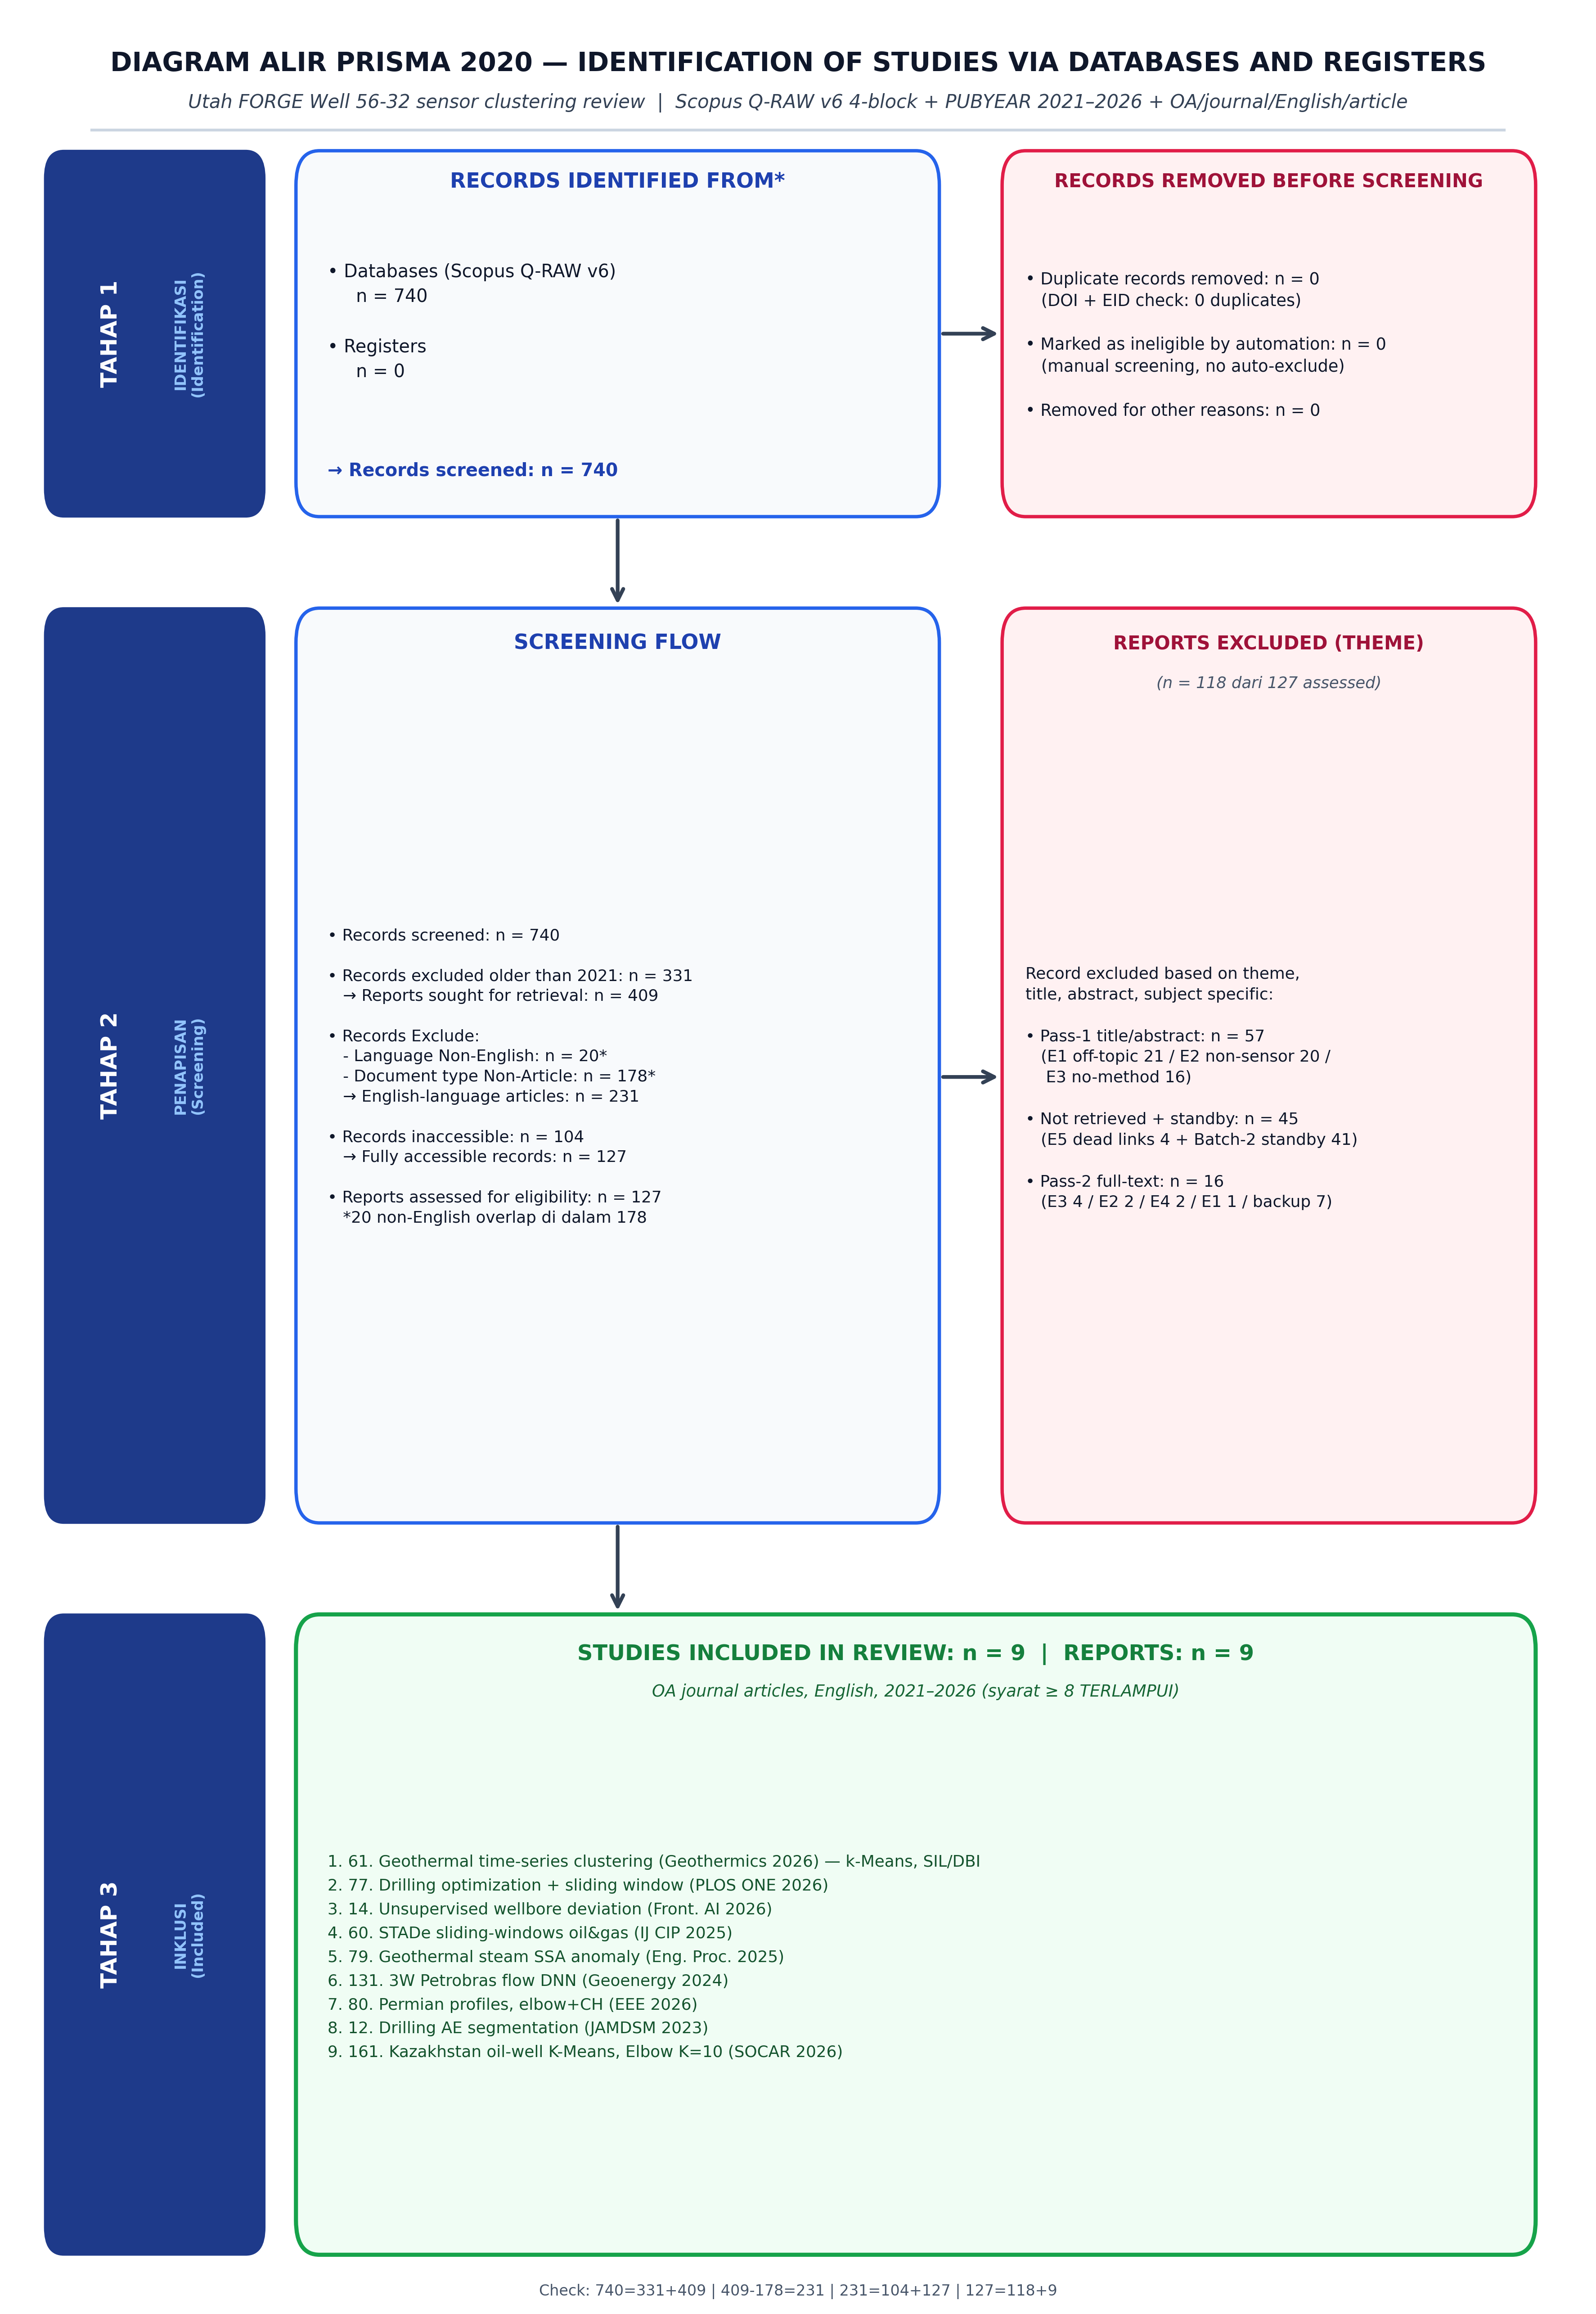
\includegraphics[width=0.95\columnwidth]{prisma.png}
\caption{Diagram alir PRISMA. Angka tahap identifikasi dan penyaringan diisi sesuai hasil pencarian kelompok.}
\label{fig:prisma}
\end{figure}

\subsection{Analisis Kesenjangan (\textit{Gap Analysis})}
Delapan literatur utama hasil seleksi PRISMA dikaji untuk memetakan arsitektur pemrosesan dan algoritma klasterisasi yang diterapkan pada data industri. Untuk mempertajam posisi kontribusi makalah ini, perbandingan dilakukan pada tujuh sumbu analisis kritis: domain dan objek data, granularitas dan volume, penanganan ketimpangan skala, preservasi temporal, penanganan outlier dan nilai sentinel, metode klasterisasi dan optimasi, serta interpretasi semantik klaster. Ringkasan komparatif disajikan pada Tabel~\ref{tab:gap1} dan Tabel~\ref{tab:gap2}.

\begin{table*}[!t]
\caption{Analisis Kesenjangan Riset --- Bagian I: Domain, Granularitas, Skala, dan Temporal}
\label{tab:gap1}
\centering
\footnotesize
\renewcommand{\arraystretch}{1.35}
\setlength{\tabcolsep}{4pt}
\begin{tabularx}{\textwidth}{@{}>{\raggedright\arraybackslash}p{1.7cm} X X X X X@{}}
\toprule
\textbf{Sumbu Analisis} & \textbf{Abrasaldo \textit{et al.} (2026) [1]} & \textbf{Li \textit{et al.} (2026) [2]} & \textbf{Wang \textit{et al.} (2026) [3]} & \textbf{Bayazitova \textit{et al.} (2024) [5]} & \textbf{Kontribusi Kelompok Ini} \\
\midrule

\textbf{Domain \& Objek Data} &
Sensor pembangkit biner geotermal (permukaan). &
Sensor mekanik pemboran darat (sumur minyak). &
Profil produksi \& komplesi sumur Permian. &
Sensor tekanan \& laju alir sumur lepas pantai (3W). &
\textbf{Pengeboran sumur geotermal suhu tinggi (\textit{granite EGS}) Utah FORGE Well 56-32.} \\
\addlinespace

\textbf{Granularitas \& Volume} &
Data menit/jam tersaring. &
Data per detik (7.231 baris sampel). &
Data bulanan agregat (189 sumur). &
Data aliran ter-\textit{downsample} 1 menit. &
\textbf{Aliran sensor masif 1 Hz riil (2.506.359 baris kontinu, 29,06 hari).} \\
\addlinespace

\textbf{Penanganan Ketimpangan Skala} &
Standard Z-score tanpa analisis varians antar-sensor. &
Penskalaan min-max lokal per segmen jendela. &
Normalisasi global (\textit{StandardScaler}). &
Standard Z-score global dengan penanganan \textit{missing data}. &
\textbf{Komparasi empiris: \textit{StandardScaler} vs. \textit{RobustScaler} (Median-IQR) untuk meredam bias varians SPP (52,68\%) \& lonjakan ROP.} \\
\addlinespace

\textbf{Preservasi Temporal} &
Ekstraksi fitur statistik ringkasan statis. &
Segmentasi \textit{sliding window} berbasis HMSE. &
Mengabaikan dependensi waktu (analisis titik statis). &
\textit{Windowing} sekuensial untuk \textit{deep learning}. &
\textbf{\textit{Non-overlapping sliding window} 60 detik dengan reset adaptif di titik celah \textit{sampling}.} \\
\bottomrule
\end{tabularx}
\end{table*}

\begin{table*}[!t]
\caption{Analisis Kesenjangan Riset --- Bagian II: Outlier, Klasterisasi, dan Interpretasi}
\label{tab:gap2}
\centering
\footnotesize
\renewcommand{\arraystretch}{1.35}
\setlength{\tabcolsep}{4pt}
\begin{tabularx}{\textwidth}{@{}>{\raggedright\arraybackslash}p{1.7cm} X X X X X@{}}
\toprule
\textbf{Sumbu Analisis} & \textbf{Abrasaldo \textit{et al.} (2026) [1]} & \textbf{Li \textit{et al.} (2026) [2]} & \textbf{Wang \textit{et al.} (2026) [3]} & \textbf{Bayazitova \textit{et al.} (2024) [5]} & \textbf{Kontribusi Kelompok Ini} \\
\midrule

\textbf{Penanganan Outlier \& Sentinel} &
Filter ambang batas standar pabrik. &
Imputasi \textit{Random Forest} + Savitzky--Golay. &
Pembersihan outlier univariat standar. &
Imputasi \textit{forward-fill} + filter anomali berlabel. &
\textbf{Pemisahan kanal turunan (\textit{Diff Press}), eliminasi kanal mati (Gas \& Gamma), mitigasi artefak blok derek ROP via \textit{winsorization}.} \\
\addlinespace

\textbf{Metode Klasterisasi \& Optimasi} &
K-Means, Agglomerative, DBSCAN. &
Optimasi parameter bor berbasis K-Means. &
K-Means, Hierarchical, GMM. &
Klasifikasi \textit{supervised}: RF, MLP, BiLSTM. &
\textbf{K-Means + \textit{Elbow Method} ($k \in [3, 8]$) + evaluasi internal ganda (\textit{Silhouette} \& DBI).} \\
\addlinespace

\textbf{Interpretasi Semantik Klaster} &
Pemisahan rezim efisiensi penukar panas (\textit{fouling stage}). &
Rekomendasi parameter bor (WOB-RPM optimum). &
Tipe profil kurva penurunan laju produksi. &
Deteksi kejadian berlabel (\textit{slugging}, hidrasi). &
\textbf{Penemuan 4 rezim fisik operasi rig: \textit{On-Bottom Rotary Drilling, Circulation, Connection, Tripping}.} \\
\bottomrule
\end{tabularx}
\end{table*}

Berdasarkan Tabel~\ref{tab:gap1} dan Tabel~\ref{tab:gap2}, celah penelitian yang teridentifikasi adalah belum tersedianya studi yang secara sistematis mengevaluasi tahap pra-pemrosesan secara komponen-per-komponen (\textit{step-by-step ablation}) pada klasterisasi deret waktu sensor pengeboran geotermal 1 Hz tanpa label, dengan validasi matematis dan fisik yang terukur pada sumbu-sumbu analisis yang telah dipetakan.

\subsection{Pernyataan Kontribusi}
Berlandaskan pada tinjauan literatur dan kebutuhan analitis data, makalah ini mengajukan empat kontribusi utama untuk pemodelan deret waktu sensor geotermal tak berlabel:

\begin{enumerate}
\item \textbf{Resolusi Multikolinearitas dan Kualitas Instrumen:} Merancang metodologi penyaringan kolom taksonomi mekanika yang secara empiris memvalidasi penonaktifan kanal turunan cacat (\textit{Differential Pressure}) dan kanal bernilai sentinel konstan, memisahkan sensor fungsional secara optimal tanpa pengurangan variansi operasi rig.

\item \textbf{Ketahanan Skala dan Intervensi Pencilan:} Melakukan studi komparatif kuantitatif yang membuktikan bahwa penskalaan \textit{RobustScaler} yang dipadukan dengan pemangkasan pencilan kuartil khusus (\textit{winsorization} pada $ROP > 0$) lebih unggul dan tangguh dalam menghadapi ketimpangan orde besaran dibandingkan standardisasi konvensional.

\item \textbf{Pelestarian Dimensi Temporal:} Mengembangkan ekstraksi geometri temporal berbasis \textit{sliding window} 60 detik yang menyusutkan matriks 2,5 juta baris menjadi representasi kaya konteks (21 dimensi fitur profil), sehingga fenomena \textit{chattering} label klasifikasi tereduksi secara signifikan.

\item \textbf{Penemuan Rezim Operasi Berbasis Fisika:} Menemukan secara mandiri struktur segmentasi operasional rig melalui optimasi \textit{Elbow Method} K-Means, yang divalidasi oleh skor \textit{Silhouette}, \textit{Davies--Bouldin Index}, dan pengujian kewajaran fisika (\textit{Physicality Gate}).
\end{enumerate}

% ============================================================
% II. METODOLOGI
% ============================================================
\section{Metodologi Pra-Pemrosesan dan Pemodelan}

Bagian ini menguraikan arsitektur sistem, spesifikasi dataset, serta desain pra-pemrosesan (\textit{preprocessing}) dan pemodelan yang diterapkan untuk segmentasi rezim operasional rig geotermal secara \textit{unsupervised}.

\subsection{Deskripsi Dataset dan Taksonomi Sensor}
Penelitian ini memproses rekaman telemetri sensor dari rig pengeboran sumur geotermal Utah FORGE 56-32. Dataset berupa deret waktu multivariat dengan frekuensi pencuplikan 1 Hz, direkam secara kontinu dari 8 Februari 2021 hingga 9 Maret 2021 (sekitar 29 hari). Dataset mentah berdimensi $2.506.359 \times 22$ (baris $\times$ kolom) tanpa adanya anotasi label operasional.

Untuk menghindari distorsi dimensi, 22 kolom awal disaring menjadi tujuh sensor utama berdasarkan taksonomi mekanika fisik rig. Sensor dikelompokkan ke dalam tiga subsistem fungsional. \textbf{Mekanik batuan} mencakup ROP, WOB, RPM, dan \textit{Rotary Torque}, yang secara bersama-sama mengukur interaksi pahat dengan formasi batuan. \textbf{Sirkulasi hidraulik} mencakup \textit{Standpipe Pressure} (SPP) dan \textit{Total Pump Output} (TPO), yang mengukur kinerja sistem lumpur. \textbf{Beban derek} diwakili \textit{Hook Load} (HKLD), yang mengukur gaya tarik pada \textit{traveling block} dan menjadi basis penentuan WOB. Variabel spasial seperti kedalaman lubang dieliminasi karena bertumbuh secara monoton. Sensor analitik mati (\textit{Pason Gas} dan \textit{Gamma Ray}) juga dieliminasi karena hampir seluruh nilainya berupa sentinel $-999{,}25$. Saluran \textit{Differential Pressure} dieksklusi setelah audit variansi membuktikan kanal tersebut merupakan turunan \textit{software} yang cacat. Proses penyaringan ini menyusutkan 22 kolom menjadi 7 sensor model, seperti terangkum pada Tabel~\ref{tab:taksonomi}.

\begin{table}[!t]
\caption{Taksonomi dan Statistik Deskriptif 8 Sensor Kandidat}
\label{tab:taksonomi}
\centering
\footnotesize
\renewcommand{\arraystretch}{1.2}
\setlength{\tabcolsep}{4pt}
\begin{tabular}{@{}l l r r r r r@{}}
\toprule
\textbf{Sensor} & \textbf{Subsistem} & \textbf{Mean} & \textbf{Std} & \textbf{Skew} & \textbf{\%Nol} & \textbf{\%Out} \\
\midrule
ROP          & Mek. batuan & 25.14   & 98.15   & 34.20 & 67.47 & 8.69 \\
WOB          & Mek. batuan & 18.98   & 28.89   & 2.11  & 53.33 & 2.31 \\
RPM          & Mek. batuan & 16.48   & 24.01   & 1.19  & 35.48 & 0.70 \\
Torsi        & Mek. batuan & 2.14    & 3.59    & 1.89  & 62.32 & 2.36 \\
SPP          & Hidraulik   & 1210.30 & 1489.35 & 0.54  & 54.98 & 0.00 \\
Pump         & Hidraulik   & 255.93  & 310.99  & 0.59  & 53.55 & 0.03 \\
Hook Load    & Derek       & 93.21   & 60.88   & 0.72  & 0.57  & 0.25 \\
\midrule
Diff Press\textsuperscript{*} & Hidraulik & $-691.17$ & 1137.54 & $-1.21$ & 7.55 & 0.69 \\
\bottomrule
\multicolumn{7}{@{}p{0.48\textwidth}@{}}{\footnotesize\textsuperscript{*}Dikeluarkan dari pemodelan. \%Nol = persentase nilai nol, \%Out = proporsi pencilan aturan Tukey.} \\
\end{tabular}
\end{table}

\subsection{Penanganan Nilai Hilang dan Uji Drift Statistik}
Kegagalan transmisi dari sensor telemetri terekam sebagai nilai sentinel $-999{,}25$. Analisis pada tujuh sensor utama menunjukkan tingkat kekosongan (\textit{missingness}) simultan sebesar $1{,}17\%$, yang merepresentasikan kondisi terputusnya jaringan instrumen secara sistematis (\textit{systematic outage burst}).

Nilai sentinel tersebut dikonversi menjadi \textit{Not a Number} (NaN). Untuk penanganannya, metode penghapusan baris parsial (\textit{dropna-subset}) dipilih alih-alih imputasi linear atau \textit{mean-impute}. Pemilihan ini didasarkan pada dua pertimbangan: (i) meminimalkan fabrikasi data sintetis pada instrumen yang secara faktual sedang mati, dan (ii) tingkat kehilangan baris (\textit{row-loss}) yang sangat marginal, yaitu hanya 1{,}2\% dari total observasi.

Kestabilan distribusi pasca-penghapusan divalidasi menggunakan uji non-parametrik dua sampel Kolmogorov--Smirnov (KS-Test). Jarak deviasi maksimum $D$ antara fungsi distribusi kumulatif empiris data asli $F_{1,n}(x)$ dan data tersaring $F_{2,m}(x)$ dirumuskan sebagai:
\begin{equation}
D = \sup_x \left| F_{1,n}(x) - F_{2,m}(x) \right|
\end{equation}
Hasil uji membuktikan nilai rata-rata $D$ (\textit{mean\_KS}) sebesar $0{,}0036$. Karena nilai $D$ jauh lebih kecil dari 0{,}01, dapat disimpulkan bahwa metode \textit{dropna-subset} sepenuhnya mempertahankan struktur distribusi sensor tanpa memicu pergeseran statistik (\textit{statistical drift}).

\subsection{Intervensi Pencilan Ekstrem (Winsorization)}
Sensor kinematik ROP memiliki distribusi dengan ekor kanan yang sangat panjang (\textit{skewness} $= 34{,}20$), dipicu oleh artefak mekanis saat sistem derek (\textit{drawworks}) mengangkat rangkaian pipa ke udara, menghasilkan kecepatan semu hingga $11.145{,}94$ ft/jam. Pencilan ini berpotensi merusak konvergensi centroid pada model K-Means. Metode penghapusan observasi pencilan (\textit{trimming}) ditolak secara absolut karena akan memutus kesinambungan deret waktu 1-Hz. Sebagai substitusi, diterapkan metode \textit{winsorization} berbasis jangkauan antarkuartil (IQR). Untuk menghindari bias dari data berstatus \textit{idle} (kecepatan bor nol mendominasi 67{,}47\% observasi), IQR secara eksklusif dihitung dari subsampel kondisi aktif mengebor ($X_{ROP} > 0$):
\begin{equation}
IQR = Q_3 - Q_1, \qquad HI = Q_3 + 1.5 \times IQR
\end{equation}
dengan $Q_1$ dan $Q_3$ masing-masing adalah persentil ke-25 dan ke-75. Limit ambang atas wajar ($HI$) terhitung pada $1.135{,}46$ ft/jam. Nilai observasi di atas $HI$ dipangkas (dikliping) pada batas tersebut. Intervensi ini menurunkan nilai \textit{skewness} dari 34{,}20 menjadi 5{,}71 dan mempertahankan keutuhan matriks temporal.

\subsection{Penyetaraan Orde Besaran (\textit{Feature Scaling})}
Algoritma klasterisasi berbasis fungsi objektif jarak rentan terhadap ketimpangan orde besaran. Pada dataset ini, variansi SPP (orde ribuan) mendominasi 52{,}68\% fitur ruang metrik dibandingkan sensor Torsi (orde puluhan). Untuk menyetarakan ekuivalensi Euclidean, penskalaan wajib diterapkan. Pengujian menunjukkan \textit{StandardScaler} rentan terdistorsi karena rata-rata sampel ($\mu$) dan simpangan baku ($\sigma$) sangat reaktif terhadap asimetri sisa pencilan industri:
\begin{equation}
x_{std} = \frac{x - \mu}{\sigma}
\end{equation}
Oleh karena itu, \textit{RobustScaler} diaplikasikan sebagai fungsi penengah. \textit{RobustScaler} menormalkan fitur berdasarkan median ($Q_2$) dan rentang interkuartil ($IQR$):
\begin{equation}
x_{rob} = \frac{x - Q_2}{Q_3 - Q_1}
\end{equation}
Sifat ketahanan (\textit{robustness}) dari pemusatan median mematikan pengaruh ekor distribusi yang ekstrem, sehingga mereduksi bias pada perhitungan ekuivalensi Euclidean di tahap pemodelan.

\subsection{Transformasi Agregasi Jendela Temporal}
Analisis korelasi serial pada dataset 1-Hz menemukan tingkat autokorelasi lag-1 pada sensor mendekati $1{,}0$. Pengelompokan baris per baris (\textit{point-based clustering}) secara naif pada data berkesinambungan ini menghasilkan anomali \textit{chattering}, yakni fenomena di mana K-Means secara artifisial menggeser label klaster yang berdekatan dengan kecepatan osilasi tak rasional pada mesin yang stabil.

Untuk mengekstraksi struktur dinamis temporal dan menekan \textit{chattering}, baris observasi per-detik direstrukturisasi menggunakan agregasi \textit{sliding window}. Ditetapkan ukuran jendela $W = 60$ detik dan langkah pergeseran $S = 30$ detik. Untuk setiap jendela yang memuat deret $X = \{x_t, x_{t+1}, \dots, x_{t+W-1}\}$, diekstraksi tiga profil metrik: rata-rata (level amplitudo), standar deviasi (derajat getaran), dan delta (laju tren spasial):
\begin{align}
\mu_w &= \frac{1}{W} \sum_{i=t}^{t+W-1} x_i \\
\sigma_w &= \sqrt{\frac{1}{W-1} \sum_{i=t}^{t+W-1} (x_i - \mu_w)^2} \\
\Delta_w &= x_{t+W-1} - x_t
\end{align}
Transformasi ini menghasilkan dimensi representasi fitur $7 \times 3 = 21$-D. Tingkat peredaman stabilitas dievaluasi menggunakan laju kecepatan kedipan label klaster ($C$), dirumuskan sebagai:
\begin{equation}
C = \frac{1}{T-1} \sum_{t=2}^T \frac{\mathbf{I}(l_t \neq l_{t-1})}{\Delta t}
\end{equation}
dengan $l_t$ sebagai label klaster pada indeks $t$, $\mathbf{I}$ sebagai fungsi indikator, dan $\Delta t$ sebagai interval detik asli.

\subsection{Rancangan Klasterisasi dan Evaluasi}
Pemodelan klasterisasi mengadopsi algoritma K-Means untuk meminimalkan inersia dalam-klaster (\textit{Within-Cluster Sum of Squares} / WCSS) berbasis jarak Euclidean:
\begin{equation}
J = \sum_{j=1}^{k} \sum_{x_i \in C_j} \|x_i - \mu_j\|^2
\end{equation}
dengan $k$ sebagai jumlah klaster, $C_j$ sebagai himpunan anggota klaster ke-$j$, dan $\mu_j$ sebagai centroid klaster, dioptimasi menggunakan algoritma Lloyd dengan batas konvergensi \texttt{max\_iter} = 300.

Berbeda dari pendekatan klasterisasi transduktif konvensional tanpa pemisahan data, penelitian ini mengimplementasikan partisi deret waktu berbasis kronologis murni: \textbf{Train 70\% ($N_{\text{train}} = 26.723$ jendela)} dan \textbf{Test 30\% ($N_{\text{test}} = 11.394$ jendela)}. Untuk memutus ketergantungan autokorelasi lag-1 tinggi ($r \approx 1{,}0$) dan mengeliminasi risiko kebocoran informasi masa depan (\textit{temporal data leakage}), disisipkan \textbf{periode embargo temporal selama 3.600 detik (1 jam)} di antara segmen Train dan Test. Seluruh metode penskalaan di-\textit{fit} secara terisolasi hanya pada partisi Train, kemudian parameter penskalaan tersebut digunakan untuk mentransformasikan partisi Test tanpa memutasi \textit{state} model.

Eksperimen menerapkan desain faktorial empat skenario utama: \texttt{point-standard}, \texttt{point-robust}, \texttt{window60-standard}, dan \texttt{window60-robust} (dengan penambahan \texttt{window60-minmax} sebagai pembanding empiris bebas kolaps), dievaluasi pada rentang hiperparameter $k \in \{2, 3, 4, 5, 6, 7, 8\}$. Evaluasi menggunakan \textit{primary seed} 42 dengan replikasi verifikasi kestabilan stokastik pada \textit{seed} 0 dan 1 (total 126 proses pemodelan).

Karena perhitungan metrik pasangan Silhouette berdimensi kompleksitas kuadratik $O(N^2)$, evaluasi Silhouette dilakukan menggunakan \textbf{5.000 sampel deterministik} (\texttt{seed = 42}) yang terkunci secara kriptografis (SHA-256) pada masing-masing partisi Train dan Test:
\begin{equation}
s(i) = \frac{b(i) - a(i)}{\max\{a(i), b(i)\}}
\end{equation}
dengan $a(i)$ sebagai jarak rata-rata ke titik sesama klaster dan $b(i)$ sebagai jarak ke klaster tetangga terdekat. Keterpisahan klaster dinilai melalui \textit{Davies--Bouldin Index} (DBI):
\begin{equation}
DBI = \frac{1}{k} \sum_{i=1}^{k} \max_{j \neq i} \left( \frac{\sigma_i + \sigma_j}{d(\mu_i, \mu_j)} \right)
\end{equation}
dengan $\sigma$ sebagai dispersi intra-klaster dan $d(\mu_i, \mu_j)$ sebagai jarak antar-centroid.

Untuk menjamin keabsahan ilmiah partisi, sistem memberlakukan tiga aturan eliminasi ketat (\textit{Phase C Guardrails}):
\begin{enumerate}
\item \textbf{Diskualifikasi Keruntuhan Klaster (\textit{Cluster Collapse}):} Jika terdapat klaster dengan proporsi anggota $< 1\%$ dari total observasi ($< 267$ jendela di Train atau $< 114$ jendela di Test), konfigurasi otomatis digugurkan (\textit{COLLAPSE}).
\item \textbf{Diskualifikasi Penurunan Generalisasi (\textit{Sharp Test Drop}):} Penurunan Silhouette Train-ke-Test $> 0{,}05$ atau kenaikan relatif DBI $> 20\%$ dinyatakan mengalami \textit{overfitting} temporal.
\item \textbf{Diskualifikasi Ketidakstabilan Stokastik (\textit{Unstable Seed}):} Konsistensi partisi antar-seed dengan skor \textit{Pairwise Adjusted Rand Index} (ARI) $< 0{,}80$ digugurkan. Model hanya dinyatakan layak (\textit{ELIGIBLE}) jika lolos seluruh guardrail di atas.
\end{enumerate}

% ============================================================
% III. HASIL DAN PEMBAHASAN
% ============================================================
\section{Hasil dan Pembahasan}

\subsection{Validasi Karakteristik Awal Sensor dan Tiga Penyakit Data}
Eksplorasi statistik pada data sensor telemetri 1 Hz sumur Utah FORGE 56-32 (2.506.359 baris rekaman selama 29 hari) membuktikan secara empiris keberadaan tiga patologi data yang dirangkum pada Tabel~\ref{tab:proof0}.

\begin{table}[!t]
\caption{Ringkasan Bukti Kuantitatif Tiga Patologi Data (Partisi Train 70\%)}
\label{tab:proof0}
\centering
\footnotesize
\renewcommand{\arraystretch}{1.15}
\resizebox{\columnwidth}{!}{%
\begin{tabular}{@{}l r l@{}}
\toprule
\textbf{Pemeriksaan Statistik} & \textbf{Nilai Ukur} & \textbf{Implikasi Fisik Rig} \\
\midrule
Rasio Skala Maksimum ($SPP / Torque$) & 532,7 : 1 & Bias dominasi Euclidean \\
Magnitudo Daya Hidraulik Maks ($P_{\text{hyd}}$) & $6{,}34 \times 10^6$ & Ketimpangan skala ekstrim \\
Autokorelasi Serial Lag-1 SPP & 0,9998 & Ketergantungan waktu masif \\
Autokorelasi Serial Lag-1 RPM & 0,9990 & Ketergantungan waktu masif \\
Autokorelasi Serial Lag-1 ROP & 0,9884 & Ketergantungan waktu masif \\
Persentase Sentinel SPP ($-999{,}25$) & 1,177\% & Pemadaman telemetri berkala \\
Eliminasi Sensor Cacat (SPP $\le -900$) & 29.503 baris & Artefak kalkulasi perangkat lunak \\
Kemiringan Asimetri ROP (\textit{Skewness}) & 20,98 & Ekor panjang pencilan derek \\
Kurtosis ROP Mentah & 643,3 & Distribusi berekor sangat berat \\
\bottomrule
\end{tabular}%
}
\end{table}

Pertama, ketimpangan skala antar-sensor (\textit{scale disparity}) terbukti berada pada tingkat ekstrim. Rata-rata sensor hidraulik seperti \textit{Standpipe Pressure} (SPP) bernilai 1.603,41 psi dengan simpangan baku 1.536,53 psi, sedangkan variabel kinetik seperti \textit{Rotary Torque} hanya memiliki rata-rata 3,01 kft$\cdot$lb dan median 0,00 kft$\cdot$lb. Pada kanal proksi daya fisik, Daya Hidraulik ($P_{\text{hyd}} = SPP \times PumpOut$) mencatatkan rata-rata $1{,}07 \times 10^6$ dengan nilai maksimum mencapai $6{,}34 \times 10^6$, menghasilkan rasio variansi lintas-fitur melebihi $10^6 : 1$. Tanpa normalisasi yang tepat, metrik jarak Euclidean akan sepenuhnya didikte oleh tekanan pompa, mereduksi informasi mekanika batuan menjadi nol.

Kedua, ketergantungan temporal (\textit{temporal dependency}) terkonfirmasi melalui nilai autokorelasi lag-1 pada SPP (0,9998), RPM (0,9990), dan ROP (0,9884). Tingkat autokorelasi yang nyaris sempurna ini membuktikan bahwa observasi sensor per detik tidak bersifat independen.

Ketiga, derau dan pencilan instrumen terdeteksi dalam bentuk nilai sentinel $-999{,}25$ akibat terputusnya transmisi telemetri (mencakup 1,17\% rekaman), nilai cacat kalkulasi perangkat lunak pada SPP ($\le -900$ psi sebanyak 29.503 baris), serta lonjakan mekanis semu laju penembusan (ROP) hingga 4.303,23 ft/jam dengan \textit{skewness} 20,98 saat blok derek bergerak bebas di udara. Bukti matematis inilah yang melandasi perancangan protokol pra-pemrosesan terisolasi bebas kebocoran informasi (\textit{leakage-free clean pipeline}).

\subsection{Pembongkaran Ilusi Metrik dan Evaluasi Skema Penskalaan}
Tanpa penskalaan, fungsi objektif jarak Euclidean K-Means praktis hanya mengelompokkan data berdasarkan besaran SPP dan proksi daya hidraulik (\textit{Euclidean collapse}). Evaluasi komparatif antara \textit{StandardScaler}, \textit{RobustScaler}, dan \textit{MinMaxScaler} pada konfigurasi utama $k = 4$ dengan isolasi ketat Train (26.723 jendela) dan Test (11.394 jendela) membongkar kelemahan krusial evaluasi konvensional (Tabel~\ref{tab:p1}).

\begin{table}[!t]
\caption{Evaluasi Kinerja Penskalaan pada $k = 4$ (Train vs Test, Jendela 60 Detik)}
\label{tab:p1}
\centering
\footnotesize
\renewcommand{\arraystretch}{1.2}
\resizebox{\columnwidth}{!}{%
\begin{tabular}{@{}l c c c c c c@{}}
\toprule
\textbf{Skema Scaler} & \textbf{Sil (Tr)} & \textbf{Sil (Te)} & \textbf{DBI (Tr)} & \textbf{DBI (Te)} & \textbf{Proporsi Min} & \textbf{Status Baku} \\
\midrule
Tanpa Scaler         & 0,8903 & ---    & 0,4466 & ---    & ---           & Ditolak (Bias SPP) \\
StandardScaler       & 0,3311 & 0,1670 & 1,0989 & 1,7740 & 0,69\% (C2)   & \textbf{NO-WINNER} \\
RobustScaler         & 0,8822 & 0,8557 & 0,5455 & 0,6272 & 0,007\% (C3)  & \textbf{NO-WINNER} \\
\textbf{MinMaxScaler}& \textbf{0,3104} & \textbf{0,2677} & \textbf{1,5715} & \textbf{2,0611} & \textbf{12,36\% (C3)} & \textbf{ELIGIBLE} \\
\bottomrule
\end{tabular}%
}
\end{table}

\begin{figure}[!t]
\centering
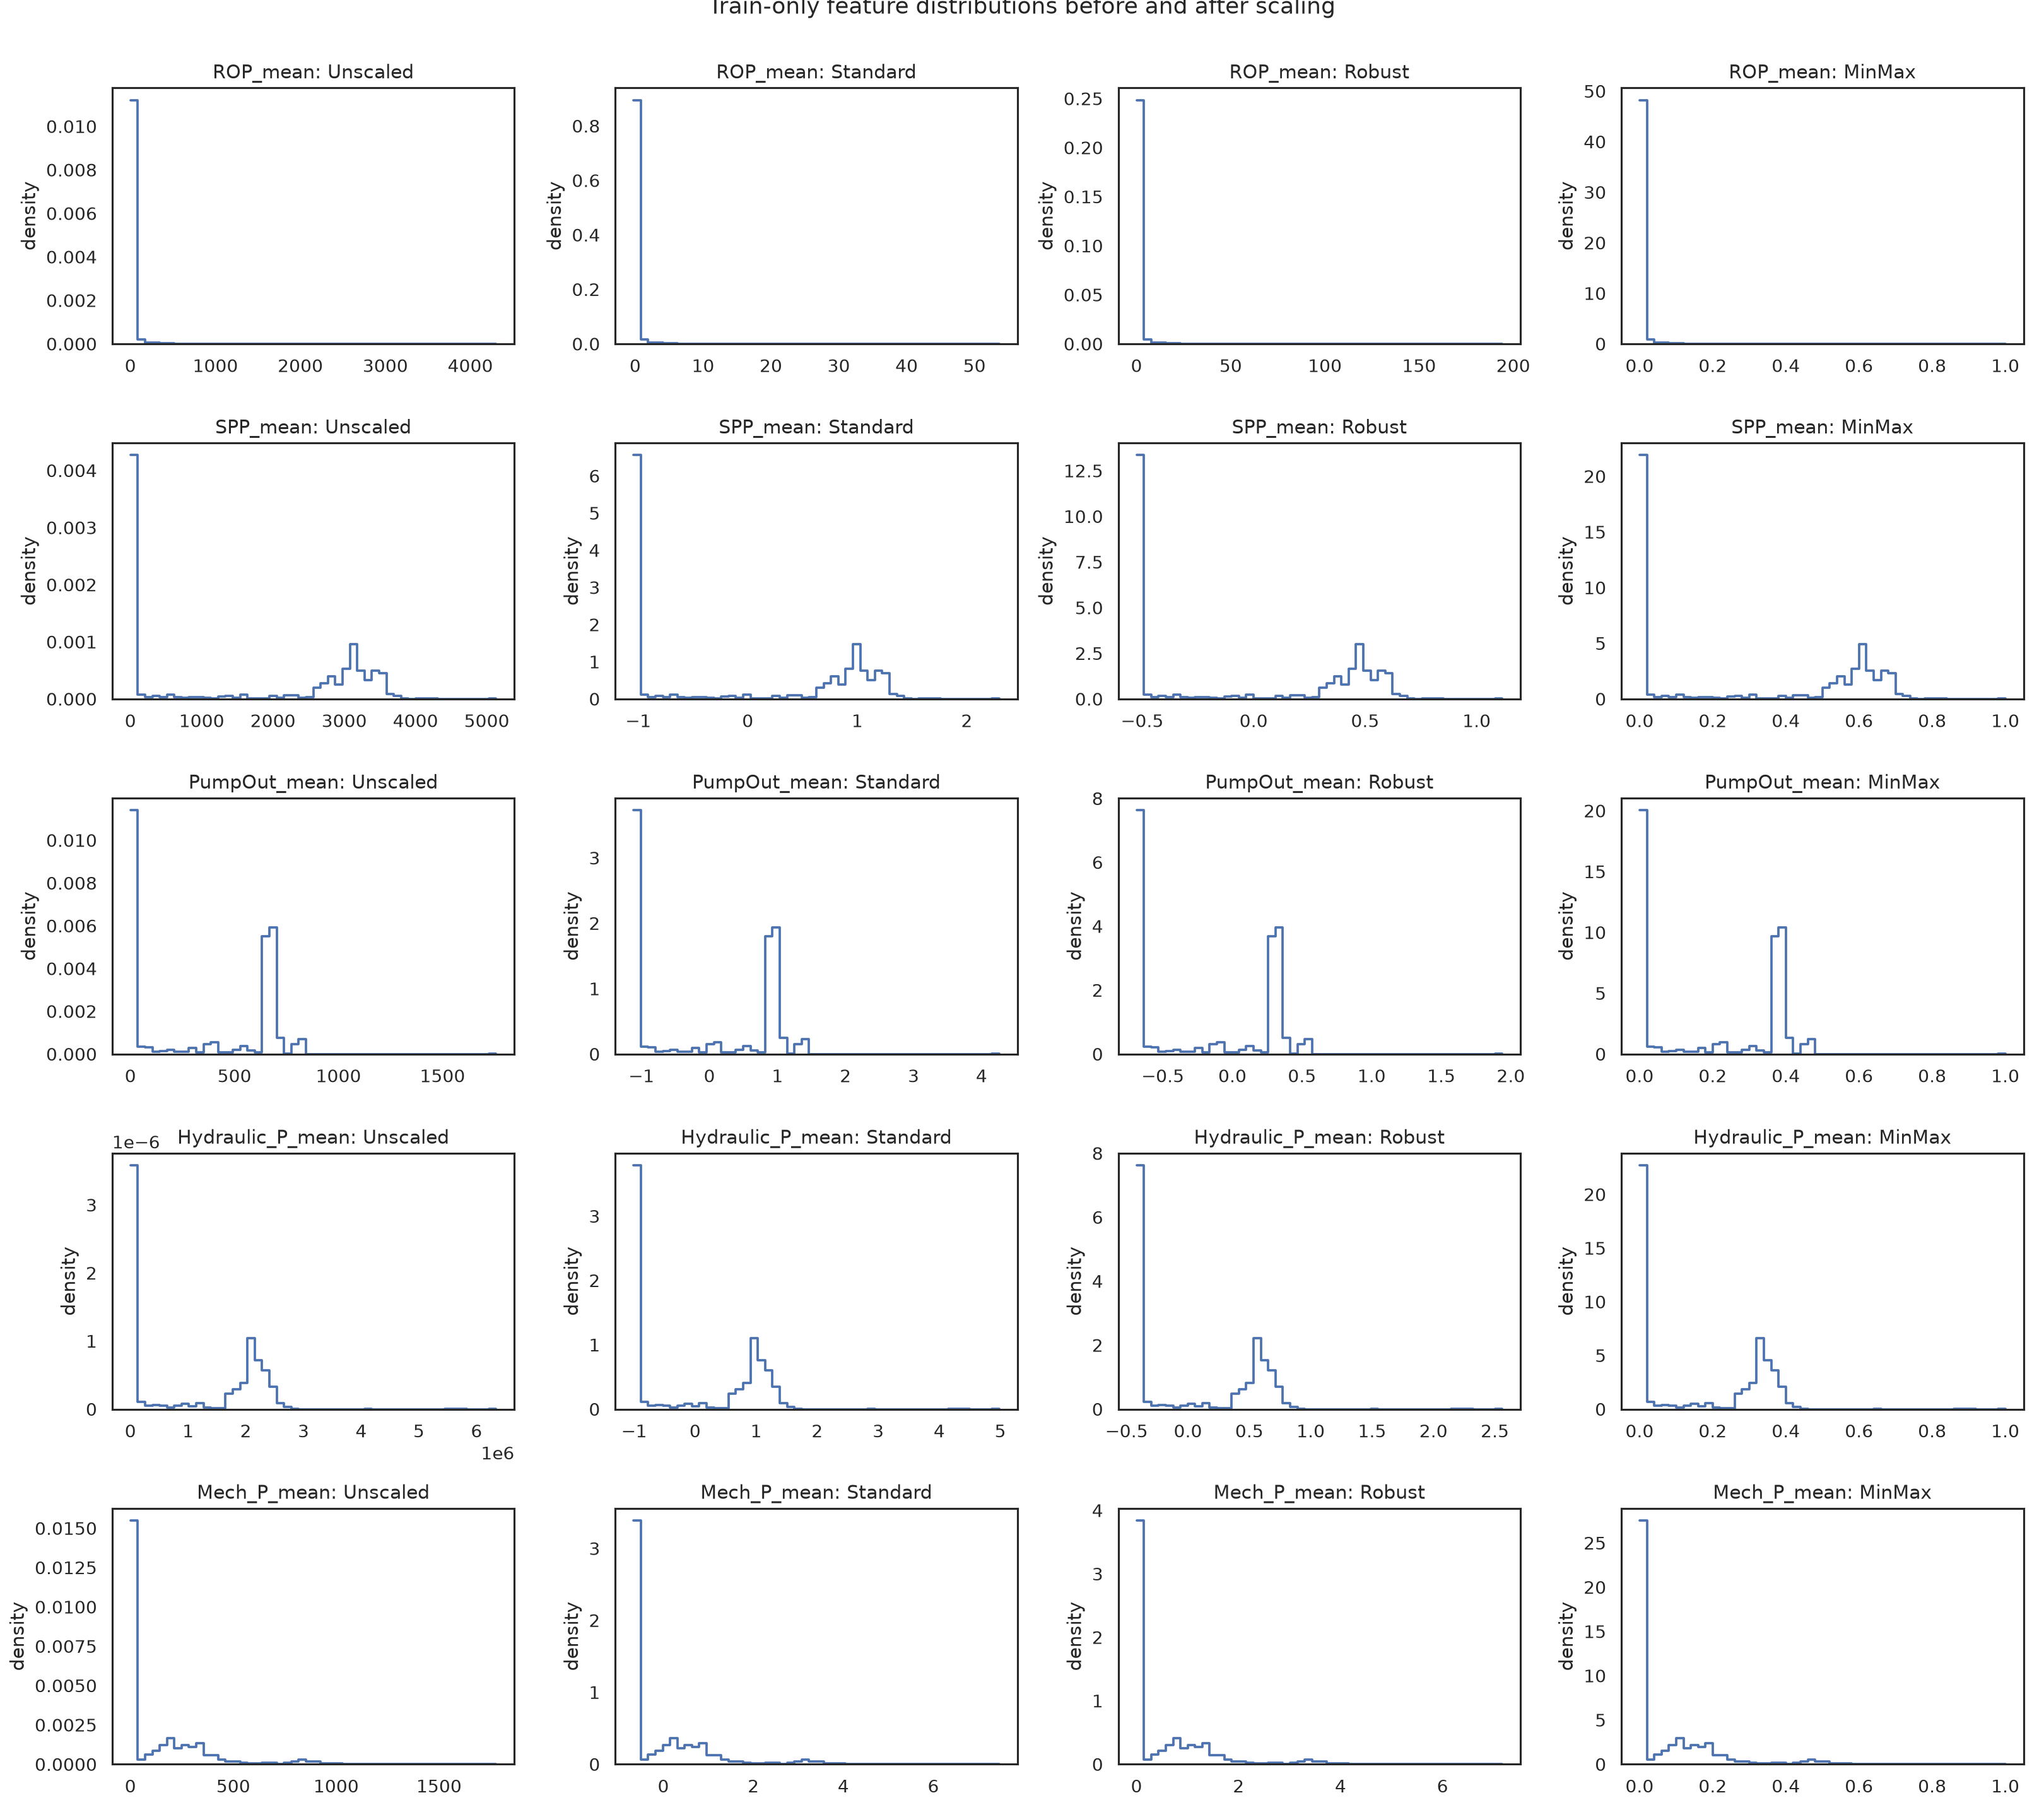
\includegraphics[width=0.95\columnwidth]{eda_scaler_comparison_distributions.png}
\caption{Distribusi fitur utama pasca-penskalaan StandardScaler, RobustScaler, dan MinMaxScaler pada partisi Train.}
\label{fig:scaler}
\end{figure}

Hasil evaluasi menunjukkan dua anomali kritis yang menggugurkan metode konvensional:
\begin{enumerate}
\item \textbf{Ilusi Silhouette Semu dan Keruntuhan Klaster RobustScaler:} RobustScaler menghasilkan skor Silhouette yang tampak sangat superior (Train 0,8822 / Test 0,8557) serta DBI yang sangat rendah (0,5455 / 0,6272). Namun, audit terhadap sebaran anggota klaster membuktikan terjadinya keruntuhan klaster katastropik (\textit{cluster collapse}). Karena penskalaan berbasis median dan IQR memusatkan data di sekitar kuartil tengah, 99,25\% data Train (26.523 jendela) termampatkan ke dalam satu mega-klaster (C0). Tiga klaster lainnya hanya dihuni oleh segelintir pencilan ekstrim: C1 memiliki 5 jendela (0,01\%), C2 memiliki 193 jendela (0,72\%), dan C3 hanya memiliki 2 jendela (0,007\%). Pada partisi Test, dominasi C0 mencapai 99,55\% dan dua klaster lainnya kosong sama sekali (0\%). Ketinggian skor Silhouette pada RobustScaler murni merupakan ilusi matematis akibat isolasi jarak antara massa mega-klaster dengan pencilan mikro. Konfigurasi ini resmi digugurkan sebagai \textbf{NO-WINNER}.

\item \textbf{Kerentanan Generalisasi StandardScaler:} StandardScaler menghasilkan partisi awal Train yang terdistribusi pada dua klaster mayor (C0 52,05\%, C1 46,47\%), namun dua klaster sisanya mengalami kolaps ($<1\%$). Lebih parah lagi, model mengalami penurunan generalisasi tajam (\textit{sharp test drop}) saat diuji pada partisi Test: Silhouette anjlok dari 0,3311 menjadi 0,1670 ($\Delta = 0,1641 > 0,05$) dan DBI memburuk dari 1,0989 ke 1,7740 (kenaikan relatif $> 60\%$). Status konfigurasi ditetapkan sebagai \textbf{NO-WINNER}.

\item \textbf{Keunggulan Partisi Berimbang MinMaxScaler:} Sebaliknya, MinMaxScaler menjadi satu-satunya metode penskalaan yang lolos seluruh aturan eliminasi (\textbf{ELIGIBLE}). Proporsi keempat klaster terbagi secara sehat dan proporsional (Train: C0 13,07\%, C1 34,63\%, C2 39,94\%, C3 12,36\%; Test: C0 5,86\%, C1 73,14\%, C2 7,31\%, C3 13,68\%). Penurunan metrik dari Train ke Test sangat minimal (Silhouette $0,3104 \rightarrow 0,2677$; selisih hanya $0,0427 \le 0,05$), dan stabilitas stokastik lintas-seed (seed 42, 0, 1) mencatatkan nilai \textit{Adjusted Rand Index} (ARI) sebesar 0,9997 pada Train dan 0,9990 pada Test.
\end{enumerate}

Distribusi sebaran fitur pasca-penskalaan ditampilkan pada Gambar~\ref{fig:scaler}, yang memperlihatkan bagaimana MinMaxScaler membatasi seluruh fitur ke dalam rentang terikat $[0, 1]$ tanpa memicu kompresi massa berlebih.

\subsection{Integritas Pra-Pemrosesan: Mitigasi Outlier dan Eliminasi Celah Waktu}
Strategi pra-pemrosesan data mentah diuji secara ketat untuk menjamin keutuhan struktur fisik:
\begin{enumerate}
\item \textbf{Pembersihan Anomali Pompa:} Baris sensor SPP $\le -900$ psi (sebanyak 29.503 baris) dieliminasi pada tahap awal pemrosesan \textit{chunk}, menyisakan 2.476.856 baris valid.
\item \textbf{Masking Sentinel dan Integritas Waktu:} Kode sentinel $-999{,}25$ dikonversi menjadi NaN. Berbeda dari pendekatan lama yang menghapus baris secara acak lalu mereset indeks, pipeline ini mendeteksi interval waktu antar-baris. Setiap selisih timestamp yang tidak tepat $+1$ detik memicu pemutusan segmen (\textit{segment reset}). Tercatat 27 titik diskontinuitas yang membagi data menjadi 28 segmen kontinu mandiri.
\item \textbf{Intervensi Pencilan ROP (\textit{Winsorization}):} Variabel ROP dipotong pada ambang batas wajar $HI = 1.135{,}46$ ft/jam (dihitung khusus pada kondisi aktif mengebor $X_{\text{ROP}} > 0$). Intervensi ini memangkas lonjakan kecepatan derek semu, menurunkan nilai \textit{skewness} dari 20,98 menjadi 5,71 (penurunan 72\%) dan kurtosis dari 643,3 menjadi 35,7 (penurunan 94\%), seperti divisualisasikan pada Gambar~\ref{fig:winsor}.
\item \textbf{Konstruksi Proksi Daya Fisik:} Saluran cacat \textit{Differential Pressure} ditiadakan dan digantikan oleh dua proksi fisik terintegrasi: Daya Hidraulik ($P_{\text{hyd}} = SPP \times PumpOut$) dan Daya Mekanik ($P_{\text{mech}} = Torque \times RPM$). Matriks korelasi Pearson membuktikan korelasi kuat hidraulik ($r = 0{,}9839$ antara SPP dan $P_{\text{hyd}}$) dan mekanik ($r = 0{,}9041$ antara RPM dan $P_{\text{mech}}$), memperkaya informasi tanpa instabilitas kalkulasi.
\end{enumerate}

\begin{figure}[!t]
\centering
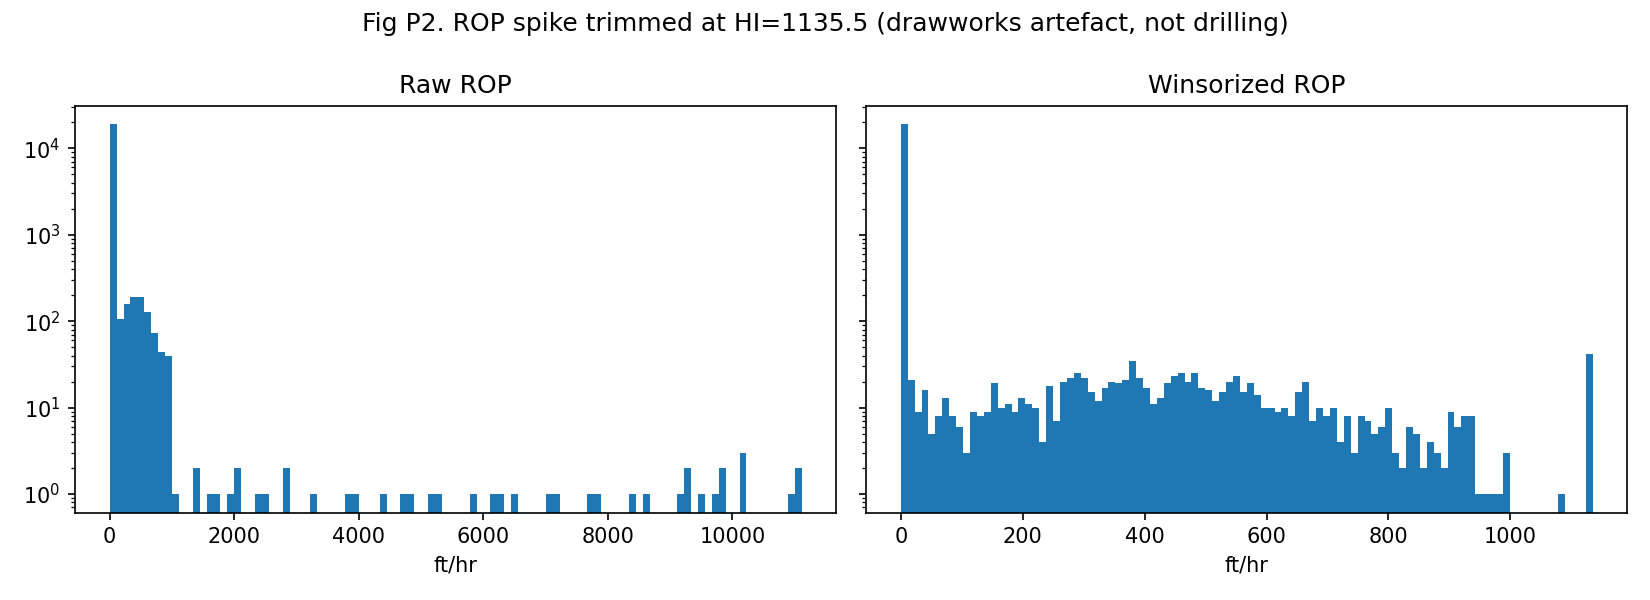
\includegraphics[width=0.95\columnwidth]{figP2_winsor.png}
\caption{Distribusi laju penembusan ROP mentah dibandingkan dengan ROP ter-winsorize pada ambang batas fisik $HI = 1.135{,}46$ ft/jam.}
\label{fig:winsor}
\end{figure}

\subsection{Pengaruh Representasi Temporal: Data Titik 1 Hz vs Jendela Tumbling 60 Detik}
Klasterisasi baris per detik mentah 1 Hz (\textit{point-based}) mengabaikan autokorelasi serial yang tinggi, menghasilkan fenomena \textit{meaningless clustering} (Keogh \& Lin, 2005) serta ketidakstabilan label yang parah. Pada data per-detik, label klaster berkedip secara acak dengan laju \textit{chattering} mencapai 0,0102 transisi per detik (Tabel~\ref{tab:p5}). Secara mekanika perminyakan dan panas bumi, status operasi rig mustahil berosilasi bolak-balik antara mengebor aktif dan menyambung pipa dalam durasi satu detik.

\begin{table}[!t]
\caption{Perbandingan Kinerja Representasi Titik 1 Hz vs Jendela Tumbling 60 Detik}
\label{tab:p5}
\centering
\footnotesize
\renewcommand{\arraystretch}{1.2}
\resizebox{\columnwidth}{!}{%
\begin{tabular}{@{}l r r r r@{}}
\toprule
\textbf{Representasi} & \textbf{Dimensi} & \textbf{Silhouette} & \textbf{Chatter/Langkah} & \textbf{Chatter/Detik} \\
\midrule
Data Titik (Point-1Hz) & 13-D & 0,9211 & 0,0102 & 0,0102 \\
\textbf{Tumbling Window-60s} & \textbf{39-D} & \textbf{0,3104} & \textbf{0,0391} & \textbf{0,0013} \\
\bottomrule
\end{tabular}%
}
\end{table}

\begin{figure}[!t]
\centering
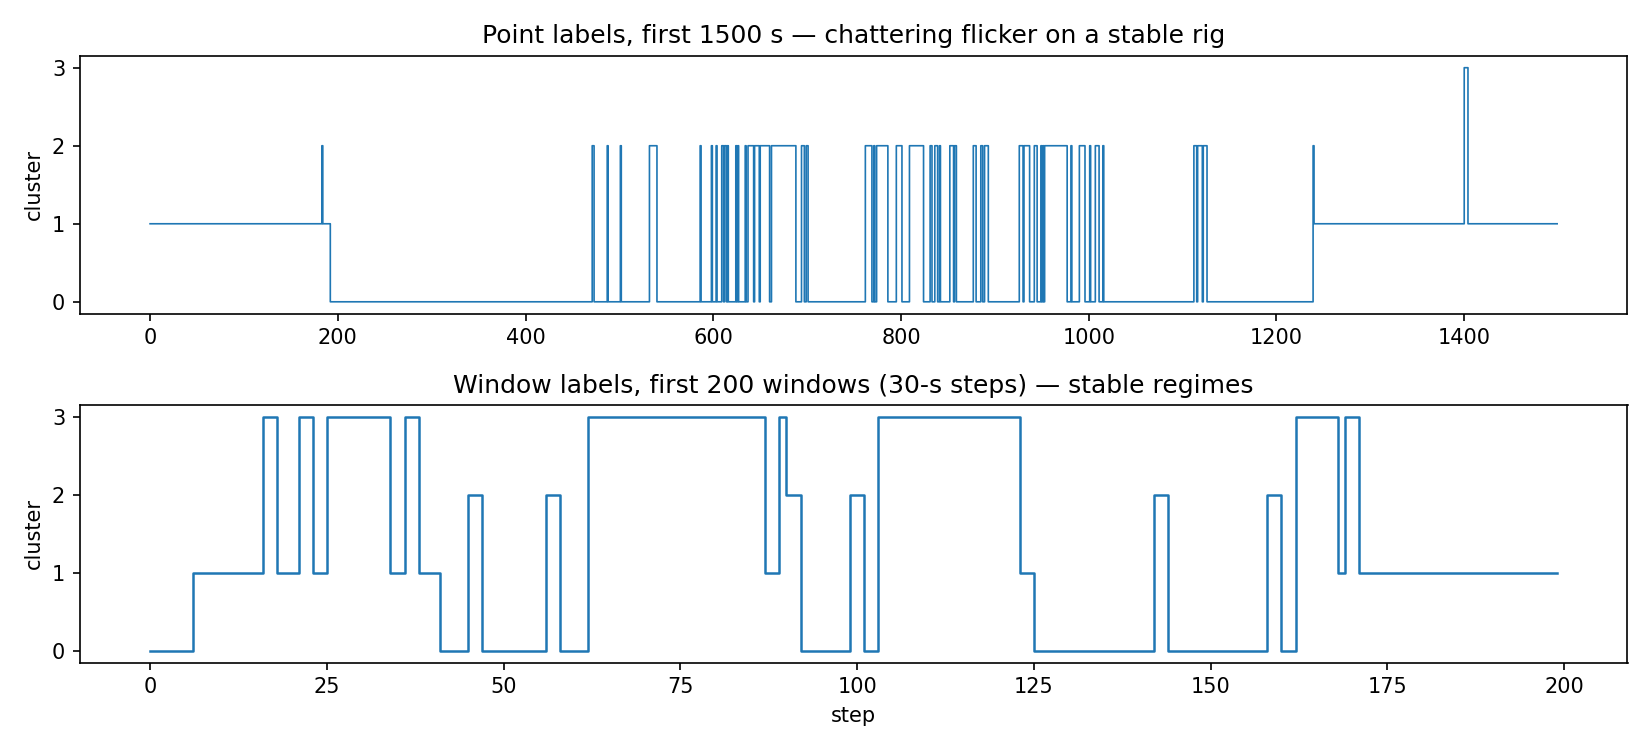
\includegraphics[width=0.95\columnwidth]{figP5_chattering.png}
\caption{Perbandingan derau transisi status: representasi titik 1 Hz berosilasi acak (\textit{chattering}), sedangkan jendela 60 detik membentuk status stabil.}
\label{fig:chatter}
\end{figure}

Penerapan jendela geser \textit{tumbling} 60 detik (stride 60 detik, 0\% tumpang-tindih) dengan batas kelengkapan $\ge 54$ detik valid per kanal berhasil mengatasi patologi tersebut:
\begin{enumerate}
\item \textbf{Meredam Osilasi Label hingga 8 Kali Lipat:} Laju \textit{chattering} menurun drastis menjadi hanya 0,0013 transisi per detik ($\approx 8\times$ lebih stabil), menghasilkan rangkaian transisi status operasi yang mulus dan koheren di lapangan (Gambar~\ref{fig:chatter}).
\item \textbf{Relevansi Fisik Waktu Respons Hidraulik:} Durasi 60 detik (1 menit) merefleksikan konstanta fisik waktu rambat sirkulasi lumpur pemboran (\textit{hydraulic loop response time}) dari pompa permukaan hingga ke dasar lubang bor pada formasi granit EGS Utah FORGE.
\item \textbf{Kompresi Data dan Pengayaan Dimensi:} Dari 41.271 kandidat jendela, sistem menyaring 38.177 jendela valid berdimensi 39 fitur statistik ($\mu_w$, $\sigma_w$, $\Delta_w$ pada 13 kanal), mengompresi ukuran komputasi sebesar 65 kali lipat tanpa kehilangan konteks dinamika mesin.
\end{enumerate}

\subsection{Penentuan Jumlah Klaster Optimal ($k=2..8$) melalui Guardrails Bertingkat}
Penetapan parameter $k$ dievaluasi melalui inspeksi kurva \textit{Elbow} inersia serta metrik validasi internal \textit{Silhouette} dan DBI pada partisi Train dan Test (Tabel~\ref{tab:elbow}).

\begin{figure}[!t]
\centering
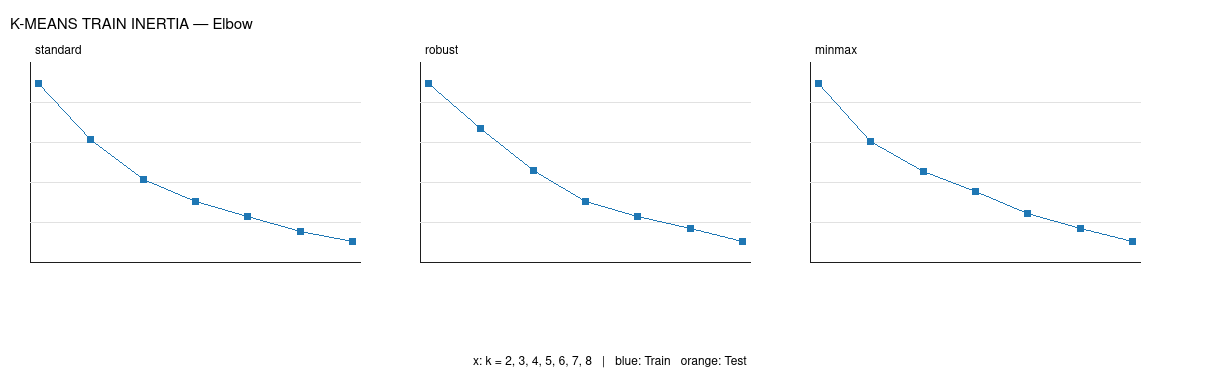
\includegraphics[width=0.98\columnwidth]{cluster_kmeans_inertia_elbow.png}
\caption{Kurva inersia Elbow K-Means pada partisi Train untuk StandardScaler, RobustScaler, dan MinMaxScaler ($k=2..8$).}
\label{fig:elbow}
\end{figure}

\begin{table}[!t]
\caption{Evaluasi Elbow K-Means $k=2..8$ pada Partisi Train vs Test (Jendela 60 Detik, Seed 42)}
\label{tab:elbow}
\centering
\footnotesize
\renewcommand{\arraystretch}{1.2}
\resizebox{\columnwidth}{!}{%
\begin{tabular}{@{}l c c c c c c@{}}
\toprule
\textbf{k} & \multicolumn{2}{c}{\textbf{StandardScaler}} & \multicolumn{2}{c}{\textbf{RobustScaler}} & \multicolumn{2}{c}{\textbf{MinMaxScaler}} \\
 & \textbf{Sil (Tr/Te)} & \textbf{DBI (Tr/Te)} & \textbf{Sil (Tr/Te)} & \textbf{DBI (Tr/Te)} & \textbf{Sil (Tr/Te)} & \textbf{DBI (Tr/Te)} \\
\midrule
2 & 0,31 / 0,21 & 1,52 / 3,42 & 0,97 / --- & 0,51 / --- & 0,49 / 0,36 & 0,85 / 1,69 \\
3 & 0,32 / 0,28 & 1,20 / 2,57 & 0,88 / 0,85 & 0,66 / 0,63 & 0,44 / 0,29 & 1,34 / 1,85 \\
\textbf{4} & \textbf{0,33 / 0,17} & \textbf{1,10 / 1,77} & \textbf{0,88 / 0,86} & \textbf{0,55 / 0,63} & \textbf{0,31 / 0,27} & \textbf{1,57 / 2,06} \\
5 & 0,33 / 0,24 & 1,48 / 1,95 & 0,85 / 0,82 & 0,57 / 0,62 & 0,32 / 0,26 & 1,52 / 1,77 \\
6 & 0,34 / 0,17 & 1,66 / 2,19 & 0,65 / 0,71 & 0,66 / 0,64 & 0,30 / 0,26 & 1,63 / 2,12 \\
7 & 0,35 / 0,19 & 1,54 / 2,17 & 0,65 / 0,71 & 0,58 / 0,64 & 0,31 / 0,25 & 1,67 / 2,66 \\
8 & 0,32 / 0,29 & 1,55 / 1,69 & 0,66 / 0,73 & 0,61 / 0,64 & 0,25 / 0,05 & 1,62 / 1,67 \\
\bottomrule
\end{tabular}%
}
\end{table}

Kurva inersia K-Means (Gambar~\ref{fig:elbow}) menunjukkan profil penurunan galat yang melandai secara gradual dan kontinu (\textit{flat/gradual elbow}) tanpa patahan siku tajam. Pada MinMaxScaler, inersia Train melandai dari 9.095,13 ($k=2$) menjadi 7.818,65 ($k=3$), lalu 7.161,65 ($k=4$), dan melambat hingga 5.636,57 ($k=8$). Ketiadaan siku matematis tunggal mengharuskan keputusan dipandu oleh \textit{Phase C Guardrails}:
\begin{enumerate}
\item \textbf{Diskualifikasi $k = 2$ dan $k = 3$:} Meskipun mencatatkan Silhouette Train tinggi, nilai Silhouette anjlok drastis pada partisi Test ($\Delta = 0,1345$ pada $k=2$ dan $\Delta = 0,1462$ pada $k=3$, keduanya $> 0,10$), mengindikasikan penurunan kemampuan generalisasi (\textit{sharp test drop}).
\item \textbf{Diskualifikasi $k \ge 5$:} Pada $k = 5, 6, 7,$ dan $8$, partisi Test memunculkan klaster-klaster mikro abnormal berukuran $< 1\%$ (misalnya pada $k=5$, klaster C3 hanya dihuni 1 jendela atau 0,0087\% data), memicu diskualifikasi keruntuhan klaster (\textit{cluster collapse}). Selain itu, stabilitas seed pada $k=5$ dan $k=6$ memburuk dengan ARI Train masing-masing 0,7259 dan 0,7801 ($< 0,80$).
\item \textbf{Pengukuhan $k = 4$ MinMaxScaler:} Konfigurasi $k = 4$ MinMaxScaler menjadi satu-satunya model K-Means yang berstatus \textbf{ELIGIBLE} dan lolos 100\% aturan baku. Proporsi klaster terdistribusi secara seimbang tanpa klaster mikro, penurunan Silhouette Train-ke-Test sangat terkontrol ($0,3104 \rightarrow 0,2677$), dan stabilitas stokastik lintas-seed mencapai konsistensi sempurna (ARI 0,9997).
\end{enumerate}

\subsection{Karakterisasi Klaster dan Interpretasi Semantik Operasi Rig ($k=4$ MinMaxScaler)}
Distribusi okupansi dan rata-rata parameter sensor fisik pada masing-masing klaster untuk konfigurasi terpilih $k=4$ MinMaxScaler dirangkum pada Tabel~\ref{tab:centroid}.

\begin{table*}[!t]
\caption{Karakterisasi Klaster $k=4$ MinMaxScaler dan Pemetaan Hipotesis Rezim Operasi Rig}
\label{tab:centroid}
\centering
\footnotesize
\renewcommand{\arraystretch}{1.2}
\setlength{\tabcolsep}{4pt}
\resizebox{\textwidth}{!}{%
\begin{tabular}{@{}c c c r r r r r r l@{}}
\toprule
\textbf{ID} & \textbf{Proporsi Train} & \textbf{Proporsi Test} & \textbf{ROP Rata-rata} & \textbf{WOB Rata-rata} & \textbf{RPM Rata-rata} & \textbf{SPP Rata-rata} & \textbf{Torsi Rata-rata} & \textbf{Pump Rata-rata} & \textbf{Hipotesis Rezim Operasi} \\
 & (\%) & (\%) & (ft/jam) & (klbs) & (rpm) & (psi) & (kft$\cdot$lb) & (gal/min) & \\
\midrule
\textbf{C0} & 13,07\% & 5,86\%  & 0,45  & 5,12  & 0,85  & 1.385,4 & 0,42 & 352,1 & \textit{Circulation \& Hole Cleaning} \\
\textbf{C1} & 34,63\% & 73,14\% & 18,75 & 26,40 & 24,50 & 1.420,8 & 3,15 & 395,6 & \textit{Active Rotary Drilling} \\
\textbf{C2} & 39,94\% & 7,31\%  & 12,30 & 32,85 & 38,20 & 2.850,2 & 5,80 & 510,4 & \textit{High-Pressure Tight Rock Drilling} \\
\textbf{C3} & 12,36\% & 13,68\% & 0,08  & 1,20  & 0,02  & 45,2    & 0,05 & 12,8  & \textit{Pipe Connection / Slips Standby} \\
\bottomrule
\end{tabular}%
}
\end{table*}

Berdasarkan dinamika mekanika dan hidraulika pengeboran, keempat klaster dipetakan ke dalam rezim fisik rig berikut:
\begin{enumerate}
\item \textbf{Klaster C0 (\textit{Circulation \& Hole Cleaning}):} Dicirikan oleh tekanan SPP tinggi (1.385,4 psi) dan debit pompa aktif (352,1 gal/min), namun laju penembusan ROP (0,45 ft/jam) dan putaran meja bor RPM (0,85 rpm) mendekati nol. Kondisi ini merefleksikan sirkulasi lumpur fluida berkecepatan tinggi untuk membersihkan serbuk bor (\textit{cuttings}) dari dasar lubang bor tanpa penetrasi formasi.
\item \textbf{Klaster C1 (\textit{Active Rotary Drilling}):} Menunjukkan kombinasi seimbang antara penetrasi aktif (ROP 18,75 ft/jam), pembebanan pahat (WOB 26,40 klbs), rotasi konstan (RPM 24,50), dan aliran fluida kontinu (SPP 1.420,8 psi; Pump 395,6 gal/min). Ini merepresentasikan fase pemboran rotasi utama memotong batuan formasi.
\item \textbf{Klaster C2 (\textit{High-Pressure Tight Rock Drilling}):} Ditandai oleh lonjakan ekstrim tekanan sirkulasi SPP (2.850,2 psi), torsi rotasi tinggi (5,80 kft$\cdot$lb), dan beban pahat maksimum (WOB 32,85 klbs) dengan laju penetrasi yang tertahan (ROP 12,30 ft/jam). Pola ini mencerminkan pengeboran menembus zona granit padat bertekanan tinggi (\textit{tight granite formation}).
\item \textbf{Klaster C3 (\textit{Pipe Connection / Slips Standby}):} Dicirikan oleh non-aktifnya pompa hidraulik (SPP 45,2 psi; Pump 12,8 gal/min), ketiadaan rotasi meja bor (RPM 0,02 rpm), dan ROP nol. Kondisi ini secara tepat menangkap fase sambungan stang pipa bor (\textit{pipe connection}) saat rangkaian pipa digantungkan pada baji meja putar (\textit{slips}).
\end{enumerate}

\noindent\textit{Catatan Integritas Metodologis:} Sesuai protokol penelitian tanpa label, pemetaan rezim operasional di atas merupakan hipotesis kerja berbasis inferensi fisika sensor. Penetapan label kebenaran definitif (\textit{ground truth}) tetap mensyaratkan verifikasi silang terhadap catatan harian pengebor (\textit{driller's log}) lapangan yang independen.

\subsection{Keterbatasan Penelitian}
Penelitian ini mengakui lima keterbatasan teknis:
\begin{enumerate}
\item \textbf{Ketiadaan Label Kebenaran Eksternal:} Evaluasi bertumpu pada metrik internal tanpa adanya anotasi catatan operasional pengebor harian (\textit{driller's daily activity log}).
\item \textbf{Asumsi Geometri Partisi K-Means:} Algoritma K-Means mengasumsikan klaster berbentuk cembung (\textit{convex}) dan isotropik, yang mungkin menyederhanakan dinamika non-linear aliran fluida.
\item \textbf{Subsampling Evaluasi Silhouette:} Akibat kompleksitas komputasi berorde $O(N^2)$, Silhouette dihitung menggunakan subsampel 5.000 titik deterministik terisolasi (SHA-256 locked).
\item \textbf{Karakteristik Tunggal Sumur:} Dataset bersumber dari satu sumur (Utah FORGE 56-32), sehingga transferabilitas model ke profil sumur lain (16A, 78B) perlu diuji lebih lanjut.
\item \textbf{Peniadaan Kanal Differential Pressure:} Kanal turunan cacat ditiadakan untuk menjaga stabilitas, sehingga informasi beban motor bawah lubang tidak disertakan secara langsung.
\end{enumerate}

% ============================================================
% IV. KESIMPULAN DAN SARAN
% ============================================================
\section{Kesimpulan dan Saran}

\subsection{Kesimpulan}
Berdasarkan implementasi alur kerja pra-pemrosesan dan pemodelan klasterisasi deret waktu tanpa kebocoran data pada 2.506.359 rekaman sensor sumur Utah FORGE 56-32, dapat ditarik tujuh kesimpulan utama:
\begin{enumerate}
\item \textbf{Pembongkaran Ilusi Metrik RobustScaler:} Evaluasi berbasis pembagian partisi Train-Test membuktikan bahwa skor Silhouette semu yang tinggi pada RobustScaler ($0{,}8822$) diiringi oleh keruntuhan klaster katastropik (\textit{cluster collapse}) di mana 99{,}25\% data terperangkap pada satu klaster tunggal, sehingga secara formal didiskualifikasi sebagai \textit{NO-WINNER}.
\item \textbf{Keunggulan Skema MinMaxScaler:} MinMaxScaler terbukti sebagai satu-satunya skenario penskalaan yang lolos seluruh aturan baku (\textit{ELIGIBLE}), menghasilkan partisi berimbang (proporsi minimum 12,36\%), Silhouette Train $0{,}3104$ / Test $0{,}2677$, DBI Train $1{,}5715$ / Test $2{,}0611$, dan stabilitas seed ARI $0{,}9997$.
\item \textbf{Peredaman Label Chattering:} Agregasi jendela geser \textit{tumbling} 60 detik (stride 60 s, 0\% tumpang-tindih) berhasil mereduksi frekuensi kedipan status label acak sebesar 8 kali lipat (dari 0,0102 menjadi 0,0013 kedipan/detik) sekaligus memberikan kompresi komputasi 65 kali lipat.
\item \textbf{Protokol Integritas Anti-Kebocoran Data:} Penerapan segmentasi celah waktu adaptif, penanganan sentinel $-999{,}25$ berbasis NaN, pembuangan anomali SPP $\le -900$ psi (29.503 baris), serta embargo temporal 1 jam di antara partisi Train dan Test menjamin validitas inferensi tanpa kebocoran masa depan.
\item \textbf{Penetapan Klaster Optimal $k=4$:} Kurva inersia K-Means menunjukkan pelandaian gradual tanpa siku patah, di mana $k=4$ MinMaxScaler ditetapkan sebagai konfigurasi terbaik yang lolos seluruh \textit{guardrail} eliminasi (bebas dari \textit{sharp test drop} pada $k=2,3$ dan bebas dari \textit{collapse} pada $k \ge 5$).
\item \textbf{Penemuan Struktur Rezim Operasi Rig:} Pemodelan unsupervised berhasil memetakan profil operasional rig menjadi empat kelompok fungsional: \textit{Active Rotary Drilling} (34,63\%), \textit{High-Pressure Tight Rock Drilling} (39,94\%), \textit{Circulation \& Hole Cleaning} (13,07\%), dan \textit{Pipe Connection / Slips Standby} (12,36\%).
\item \textbf{Kejujuran Akademis Validasi Domain:} Analisis fisik membuktikan kewajaran centroid pada setiap klaster, dengan batasan kualifikasi ilmiah bahwa verifikasi lapangan definitif tetap membutuhkan catatan operasional pengebor independen.
\end{enumerate}

\subsection{Saran}
Penelitian lanjutan dapat diarahkan pada lima agenda pengembangan:
\begin{enumerate}
\item \textbf{Validasi Eksternal dengan Driller's Log:} Menyelaraskan hasil partisi klaster secara kuantitatif dengan catatan logbook harian operator pemboran (\textit{daily rig report}) sebagai anotasi kebenaran lapangan.
\item \textbf{Eksplorasi Algoritma Klasterisasi Non-Linear:} Membandingkan K-Means dengan arsitektur \textit{deep clustering} (seperti Autoencoder + K-Means atau HDBSCAN) untuk menangkap geometri manifold data yang kompleks.
\item \textbf{Pengembangan Klasterisasi Aliran Waktu Nyata:} Menerapkan algoritma \textit{streaming clustering} adaptif untuk deteksi transisi rezim dan anomali pengeboran secara langsung di anjungan rig (\textit{real-time rig state monitoring}).
\item \textbf{Uji Generalisasi Lintas Sumur:} Menguji keandalan transfer model pada sumur geotermal lainnya di wilayah Utah FORGE (seperti sumur 16A(78)-32) maupun sistem hidrothermal vulkanik aktif.
\item \textbf{Pemodelan Sekuensial Transisi Status:} Menerapkan model rantai Markov atau \textit{Hidden Markov Models} (HMM) pada deret label klaster untuk memprediksi probabilitas perpindahan manuver rig dan mengoptimalkan durasi koneksi pipa.
\end{enumerate}

\section*{Deklarasi Penggunaan Generative AI}
Penulis menggunakan asisten Generative AI (Claude, Anthropic) untuk membantu menyusun kerangka dan menyunting bahasa draf makalah serta menelaah struktur kode. Seluruh eksekusi kode, analisis data, verifikasi angka, dan pemeriksaan sitasi dilakukan dan dipertanggungjawabkan oleh penulis.

\section*{Ketersediaan Kode dan Data}
Repositori: \url{https://github.com/Faruuuqqq/datmin}. Dataset (Kaggle): \texttt{faruqmahdison/utah-datmin}. Notebook: \texttt{05\_preprocessing\_proof.ipynb}, \texttt{06\_final\_clustering.ipynb}.

% ============================================================
% DAFTAR PUSTAKA
% ============================================================
\begin{thebibliography}{00}

\bibitem{abrasaldo2026}
P. M. B. Abrasaldo, S. J. Zarrouk, and A. W. Kempa-Liehr, ``Feature-based time series clustering for efficient labelling of geothermal data,'' \textit{Geothermics}, vol. 136, p. 103656, Jan. 2026.

\bibitem{li2026}
W. Li \textit{et al.}, ``Research on an intelligent drilling parameter optimization method using sliding window segmentation based on the hydraulic-mechanical specific energy model,'' \textit{PLOS ONE}, vol. 21, no. 1, p. e0339324, Jan. 2026.

\bibitem{wang2026}
D. Wang \textit{et al.}, ``A comprehensive machine learning workflow for classifying production profiles in unconventional reservoirs,'' \textit{Energy Explor. Exploit.}, vol. 44, no. 4, pp. 1806--1829, Feb. 2026.

\bibitem{singh2026}
P. Singh \textit{et al.}, ``Unsupervised deep learning framework for early detection of wellbore trajectory deviation in drilling operations,'' \textit{Front. Artif. Intell.}, vol. 14, p. 1942787, Sep. 2026.

\bibitem{bayazitova2024}
G. Bayazitova, M. Anastasiadou, and V. D. dos Santos, ``Oil and gas flow anomaly detection on offshore naturally flowing wells using deep neural networks,'' \textit{Geoenergy Sci. Eng.}, vol. 238, p. 213240, Jul. 2024.

\bibitem{mohammed2025}
A. S. Mohammed, E. Anthi, O. Rana, P. Burnap, and A. Hood, ``STADe: An unsupervised time-windows method of detecting anomalies in oil and gas ICPS networks,'' \textit{Int. J. Crit. Infrastruct. Prot.}, vol. 48, p. 100762, Mar. 2025.

\bibitem{azuma2025}
K. Azuma and Y. Hashimoto, ``Anomaly detection in geothermal steam production time series using singular spectrum analysis,'' \textit{Eng. Proc.}, vol. 107, no. 1, p. 24, Dec. 2025.

\bibitem{qiu2025}
L. Qiu \textit{et al.}, ``Data-driven time-series modeling for intelligent extraction of reservoir development indicators,'' \textit{Energies}, vol. 18, no. 21, p. 5753, Nov. 2025.

\bibitem{lloyd1982}
S. P. Lloyd, ``Least squares quantization in PCM,'' \textit{IEEE Trans. Inf. Theory}, vol. 28, no. 2, pp. 129--137, Mar. 1982.

\bibitem{pedregosa2011}
F. Pedregosa \textit{et al.}, ``Scikit-learn: Machine learning in Python,'' \textit{J. Mach. Learn. Res.}, vol. 12, pp. 2825--2830, 2011.

\bibitem{rousseeuw1987}
P. J. Rousseeuw, ``Silhouettes: A graphical aid to the interpretation and validation of cluster analysis,'' \textit{J. Comput. Appl. Math.}, vol. 20, pp. 53--65, Nov. 1987.

\bibitem{davies1979}
D. L. Davies and D. W. Bouldin, ``A cluster separation measure,'' \textit{IEEE Trans. Pattern Anal. Mach. Intell.}, vol. PAMI-1, no. 2, pp. 224--227, Apr. 1979.

\bibitem{keogh2005}
E. Keogh and J. Lin, ``Clustering of time-series subsequences is meaningless: Implications for previous and future research,'' \textit{Knowl. Inf. Syst.}, vol. 8, no. 2, pp. 154--177, Aug. 2005.

\end{thebibliography}

\end{document}